\documentclass[tikz,border=12pt]{standalone}
\usepackage[T1]{fontenc}
\usepackage{mathpazo}
\usepackage{amsmath,amssymb}
\usetikzlibrary{arrows.meta, positioning, calc, fit, decorations.pathreplacing}
\definecolor{stblue}{HTML}{7B97AD}
\definecolor{rwgold}{HTML}{B8995E}
\definecolor{sage}{HTML}{7A9A7E}
\definecolor{dkbrown}{HTML}{3D3530}
\definecolor{wmgray}{HTML}{7B7067}
\definecolor{cream}{HTML}{F9F6F0}
\definecolor{border}{HTML}{D4C9B8}
\definecolor{terracotta}{HTML}{C47A6A}
\definecolor{lavender}{HTML}{907EA0}

\begin{document}
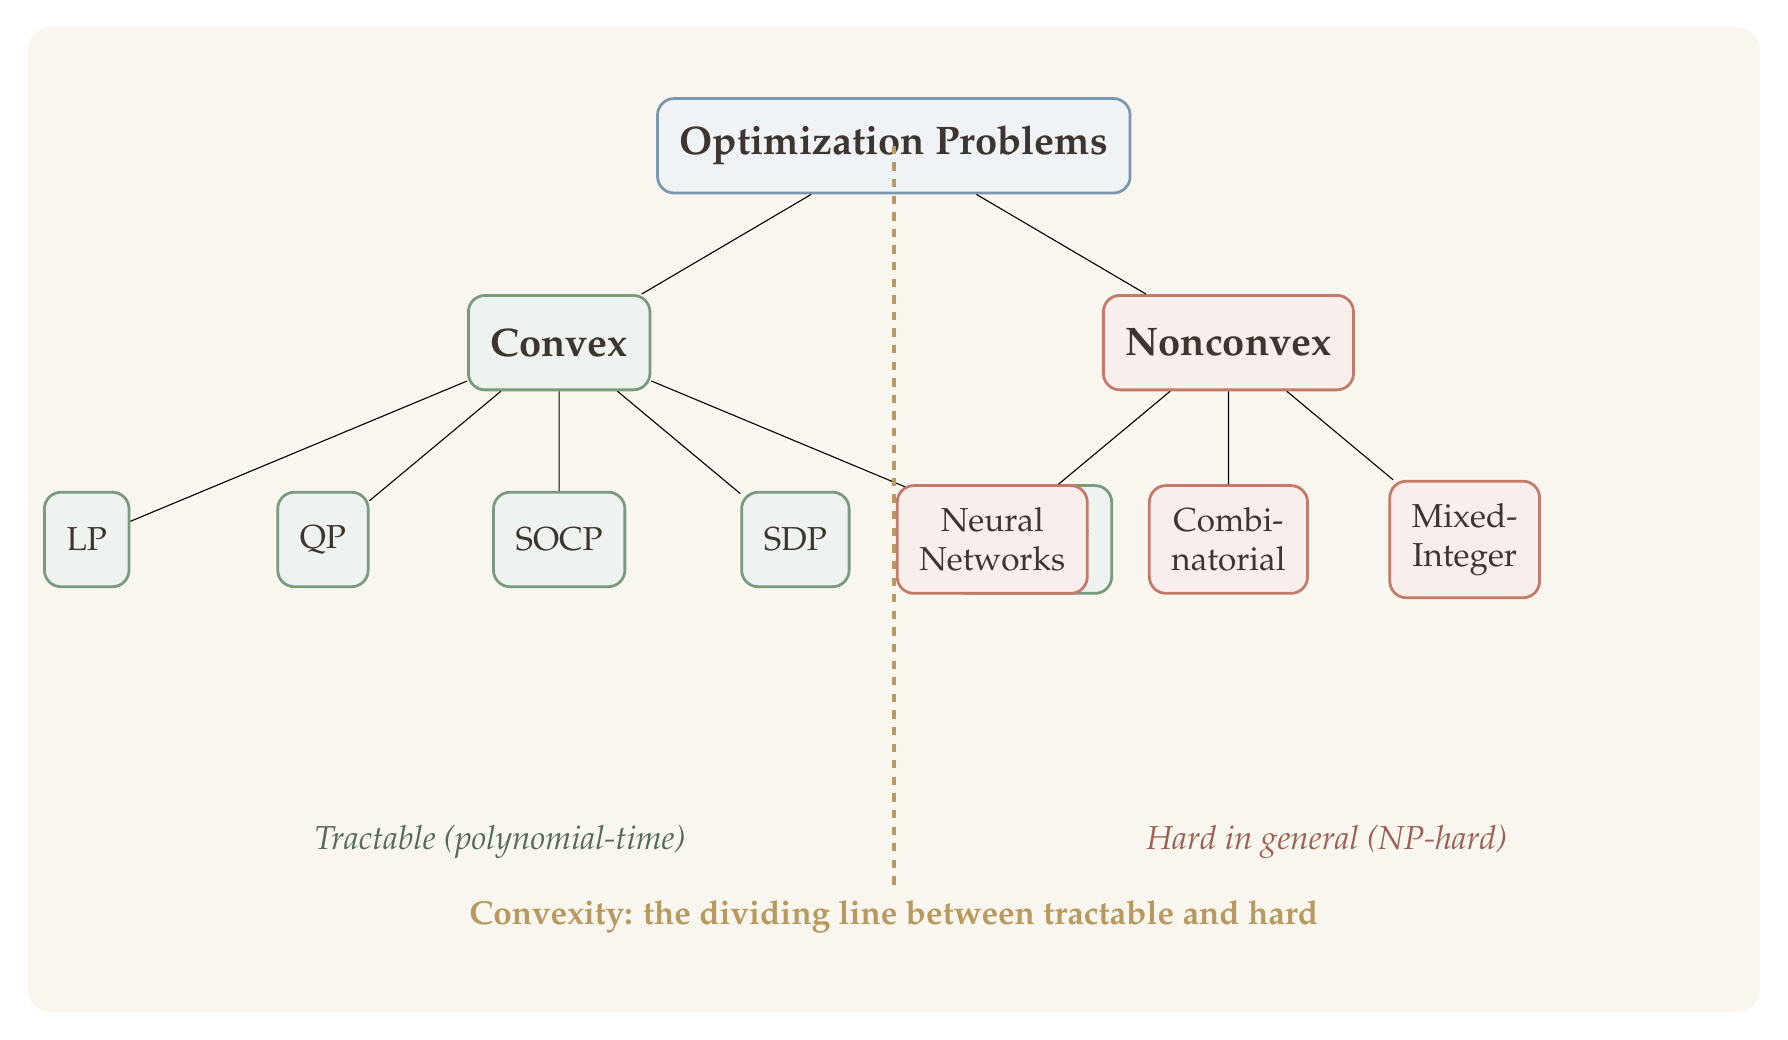
\begin{tikzpicture}[
    >={Stealth[length=4mm, width=3mm]},
    every node/.style={text=dkbrown},
    level 1/.style={sibling distance=8.5cm, level distance=2.5cm},
    level 2/.style={sibling distance=3.0cm, level distance=2.5cm},
    treenode/.style={rounded corners=6pt, inner sep=8pt, line width=1pt,
      font=\large, minimum height=1.2cm, align=center},
    convexnode/.style={treenode, fill=sage!12, draw=sage},
    nonconvexnode/.style={treenode, fill=terracotta!12, draw=terracotta},
    rootnode/.style={treenode, fill=stblue!12, draw=stblue, font=\Large\bfseries},
  ]

  % Background
  \fill[cream, rounded corners=8pt] (-11,-9) rectangle (11,3.5);

  % Tree
  \node[rootnode] (root) at (0,2.0) {Optimization Problems}
    child {
      node[convexnode, font=\Large\bfseries] (convex) {Convex}
      child { node[convexnode] (lp) {LP} }
      child { node[convexnode] (qp) {QP} }
      child { node[convexnode] (socp) {SOCP} }
      child { node[convexnode] (sdp) {SDP} }
      child { node[convexnode] (gc) {General\\Convex} }
    }
    child {
      node[nonconvexnode, font=\Large\bfseries] (nonconvex) {Nonconvex}
      child { node[nonconvexnode] (nn) {Neural\\Networks} }
      child { node[nonconvexnode] (comb) {Combi-\\natorial} }
      child { node[nonconvexnode] (mip) {Mixed-\\Integer} }
    };

  % Edges are drawn automatically by the tree, restyle them
  \tikzset{
    edge from parent/.style={draw=wmgray, line width=1pt, -},
  }

  % Tractable / Hard labels
  \node[font=\large\itshape, sage!70!black, anchor=north] at (-5.0,-6.5)
    {Tractable (polynomial-time)};
  \node[font=\large\itshape, terracotta!80!black, anchor=north] at (5.5,-6.5)
    {Hard in general (NP-hard)};

  % Dividing line annotation
  \draw[rwgold, line width=1.5pt, dashed] (0, 2.0) -- (0, -7.8);
  \node[font=\large\bfseries, rwgold, align=center, fill=cream, inner sep=5pt]
    at (0, -7.8) {Convexity: the dividing line between tractable and hard};

\end{tikzpicture}
\end{document}
